\section{Description}
\syn{SYNOPSIS}
\begin{verbatim}
	use Chart::type;     (type is one of: Bars, Composite,
	Direction, ErrorBars, HorizontalBars, Lines, LinesPoints,
	Mountain,	Pareto, Pie, Points, Split or StackedBars)
		
	$obj = Chart::type->new;
	$obj = Chart::type->new (width, height);
	
	$obj->set( $key_1, $val_1, ... , $key_n, $val_n);
	$obj->set( $key_1 => $val_1, ... , $key_n => $val_n);
	$obj->set( %hash );
	
	#GifGraph.pm-style API to produce png formatted charts
	@data = ( \@x_tick_labels, \@dataset_1, ... \@datase_n);
	$obj->png ( "filename", \@data );
	$obj->png ( $filehandle, \@data );
	$obj->png ( FILEHANDLE, \@data );
	$obj->cgi_png ();
	
	#Graph.pm-style API
	$obj->add_pt ($label, $val_1, ... $val_n);
	$obj->add_dataset ($val_1, ..., $val_n);
	$obj->png ("filename");
	$obj->png ($filehandle);
	$obj->png (FILEHANDLE);
	$obj->cgi_png();
	The similar functions are available for jpeg	
	
	#Retrieve imagemap information
	$obj->set('imagemap' => 'true' );
	$imagemap_ref = $obj->imagemap_dump();
	
\end{verbatim}
\clearpage
The Perl module \fett{Chart} creates png or jpeg Files with charts. Chart can also create dynamic charts for web sites.\\
It is possible to create a lot of different chart types with Chart: Bars, Composite, Direction, ErrorBars, HorizontalBars, Lines, LinesPoints, Mountain, Pareto, Pie, Points, Split, StackedBars.\\
Take a look at their descriptions to see how they work. All of the special types are classes by them self. All this classes have the same abstract superclass: Base.pm. The hierarchy of Chart is shown in Figure 1.      
\begin{figure}[h]
	\begin{center}
		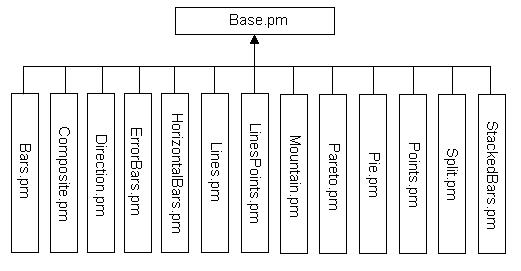
\includegraphics[scale=0.5]{Aufbau.png}
	\end{center}
	\caption{The hierarchy of chart}
	\label{fig:Aufbau}
\end{figure}
Therefore you have to create an \fett{instance of one of the subclasses}, to get a chart object.\\
All of the methods and most of the options chart provides, are implemented in Base. But the drawing of the graph itself happens in the respective subclass. Figure 2 shows the Elements of an chart object.\\  
\begin{figure}[h]
	\begin{center}
		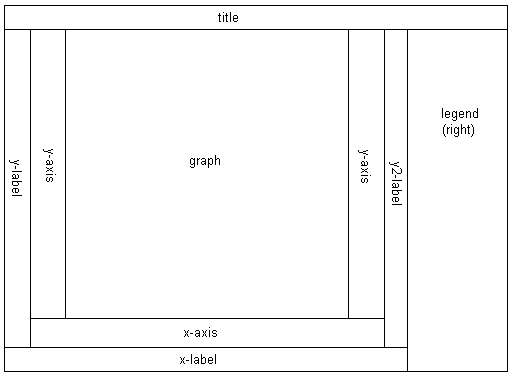
\includegraphics[scale=0.4]{../latex/Bericht/Elemente.png}
	\end{center}
	\caption{Elements of a chart}
	\label{fig:Elemente}
\end{figure}
The graph area in the middle is draw by the subclass, all other Elements are drawn by Base. But some classes don`t need all of this elements or need special elements. Then those elements had to be over written in the respective class. For Example the class Pie doesn't need axes, so the methods for drawing the axes in Base.pm are over written by methods in Pie.pm, which draw nothing. Furthermore the legend in a pie chart are a little bit different. Therefore Pie.pm has own methods for drawing the legends. But these things are managed by Chart. You don't have to attend to it. \par
Chart uses Lincoln Stein's GD module for all its graphics primitives calls. So you need a installed version of GD.pm to use Chart. This module is like Chart available in the CPAN online archive at \kursiv{http://www.cpan.org/}. \\       